\documentclass[11pt,letterpaper]{article}
\usepackage[utf8]{inputenc}
\usepackage[top=1in,bottom=1in,left=1in,right=1in]{geometry}
\usepackage{amsmath}
\usepackage{amsfonts}
\usepackage{amssymb}
\usepackage{amsthm}
\usepackage{bm}
\usepackage{braket}
\usepackage{cancel}
\usepackage{enumitem}
\usepackage{float}
\usepackage{graphicx}
\usepackage{hyperref}
\usepackage{mathabx}
\usepackage{parskip}
\usepackage{tensor}
\usepackage{titlesec}
\usepackage{titling}
\usepackage{listings}


\setenumerate{leftmargin=*,label=\bf(\alph*)}


\titlelabel{(\thetitle)\quad}
\titleformat*{\section}{\large\bfseries}
\titleformat*{\subsection}{\normalsize\bfseries}
\setlength{\droptitle}{-5em}



\let\Re\relax
\DeclareMathOperator{\Re}{Re}
\let\Im\relax
\DeclareMathOperator{\Im}{Im}

\DeclareMathOperator*{\argmax}{arg\,max}
\DeclareMathOperator*{\argmin}{arg\,min}


\newcommand{\bhat}[1]{\hat{\bm{#1}}}


\renewcommand{\thesubsection}{\normalsize \alph{subsection}}
\renewcommand{\d}{\mathrm{d}}
\renewcommand{\vec}[1]{\bm{#1}}
\newcommand{\del}{\vec{\nabla}}
\newcommand{\e}{\epsilon}
\newcommand{\tpd}[3]{\left( \frac{\partial #1}{\partial #2} \right)_{#3}}
\newcommand{\pd}[2]{\frac{\partial #1}{\partial #2}}
\newcommand{\spd}[2]{\frac{\partial^2 #1}{\partial {#2}^2}}
\def\dbar{{\mathchar'26\mkern-12mu d}}

\allowdisplaybreaks


\author{Sam Kowash}
\numberwithin{equation}{section}
\numberwithin{figure}{section}
\title{CSE 546 HW \#1}

\begin{document}
\maketitle
\section{Gaussians}

\begin{figure}[H]
	\centering
	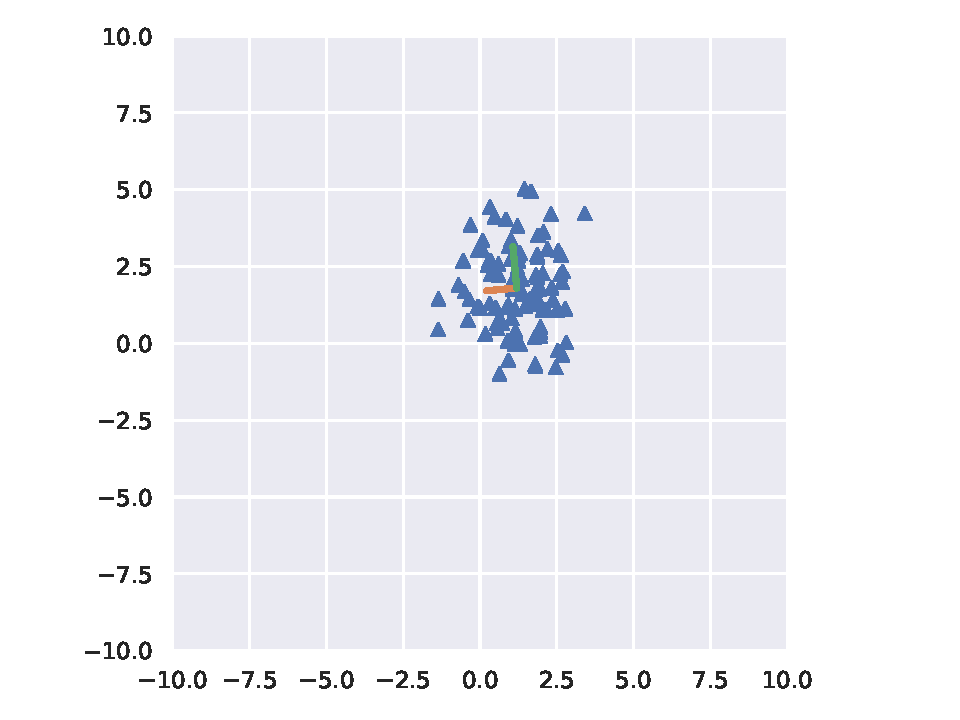
\includegraphics[width=.6\textwidth]{figures/plot_0.pdf}
\end{figure}

\begin{figure}[H]
	\centering
	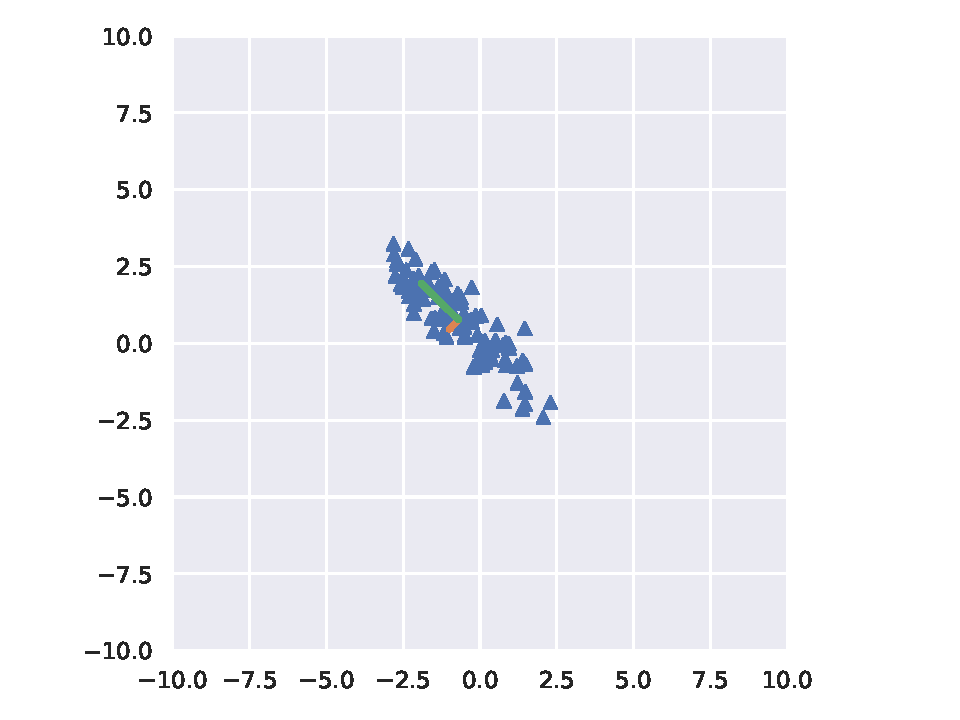
\includegraphics[width=.6\textwidth]{figures/plot_1.pdf}
\end{figure}

\begin{figure}[H]
	\centering
	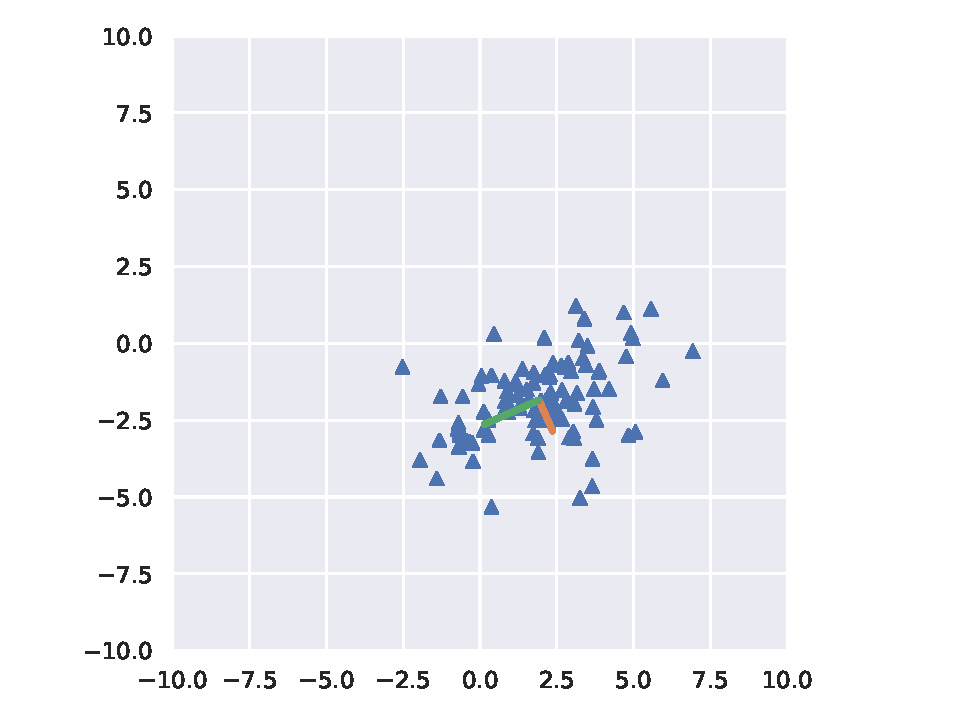
\includegraphics[width=.6\textwidth]{figures/plot_2.pdf}
\end{figure}


\section{MLE and bias--variance tradeoff}

\begin{enumerate}[label=\arabic*.]
	\setcounter{enumi}{1}
	\item If we draw $x_1,\ldots,x_n \sim \text{uniform}(0,\theta)$ for some positive parameter $\theta$, then
	\begin{align*}
		\mathbb{P}(x_1,\ldots,x_n \mid \theta) &= \left\{\begin{array}{ll}
			\left(\frac{1}{\theta}\right)^n & \text{if } x_1,\ldots,x_n \in [0,\theta]\\
			0 & \text{else}\\
			\end{array}\right.
	\end{align*}
	%
	We can see that the likelihood increases as $\theta$ decreases as long as all points drawn still lie in $[0,\theta]$, so we conclude that the MLE is $\hat{\theta} = \max(x_1,\ldots,x_n)$.




	\item Let $(x_1,y_1),\ldots,(x_n,y_n) \in \mathbb{R}^d \times \mathbb{R}$ be drawn from some population. We define
	%
	\begin{align*}
	\hat{w} = \argmin_{w} \sum_{i=1}^n (y_i - w^T x_i)^2.
	\end{align*}
	%
	Let $(\tilde{x}_1,\tilde{y}_1),\ldots,(\tilde{x}_m,\tilde{y}_m)$ be test data drawn from the same population. We define the training and test losses
	%
	\begin{align*}
		R_\mathrm{tr} &= \frac{1}{n} \sum_{i=1}^n \left(y_i - \hat{w}^T x_i\right)^2,&
		R_\mathrm{te} &= \frac{1}{m} \sum_{i=1}^n \left(\tilde{y}_i - \hat{w}^T \tilde{x}_i\right)^2.
	\end{align*}
	%
	We are interested in comparing the expected values of these losses over all possible training and test draws. Note that because our points are drawn i.i.d., each term in $R_\mathrm{tr}$ should make the same expected contribution and each term in $R_\mathrm{te}$ should make the same expected contribution (this is to say that in the expectation, $\hat{w}$ should not ``prefer'' any particular data direction). Thus without loss of generality we can analyze the case $m=n$. \ldots
\end{enumerate}









\section{Ridge regression on MNIST}

\begin{enumerate}[label=\arabic*.]
	\setcounter{enumi}{4}
	\item We develop a least-squares classifier for the MNIST handwritten digit set.
	\begin{enumerate}
	\item We want to minimize the objective
	%
	\begin{align*}
		\widehat{W} &= \argmin_{W \in \mathbb{R}^{d \times k}} \sum_{i=0}^n \|W^T x_i - y_i \|_2^2 + \lambda \|W\|_F^2,
	\end{align*}
	%
	but have run out of time to show that the answer is $(X^T X + \lambda I_d)^{-1} X^T Y$.



	\item Nothing reportable in this part.



	\item Using the pixels directly as features, we obtained a test error of 13.97\%. Code not included because it's a boring subset of the code that is included.



	\item We obtained a better feature set through the transform
	%
	\begin{align*}
		h(x) &= \cos\left(G x + b\right),
	\end{align*}
	%
	where $G$ is a $p \times d$ matrix with entries drawn i.i.d. from $\mathcal{N}(0,0.1)$ and $b$ is a length $p$ vector drawn from a uniform distribution on $[0,2\pi)$. We applied single-sample cross-validation with an 80/20 split to optimize the selection of $p$, measuring training and validation errors for 371 values ranging from 1 to 23000. The results are displayed in Fig.~\ref{fig:val}.

	\begin{figure}[H]
		\centering
		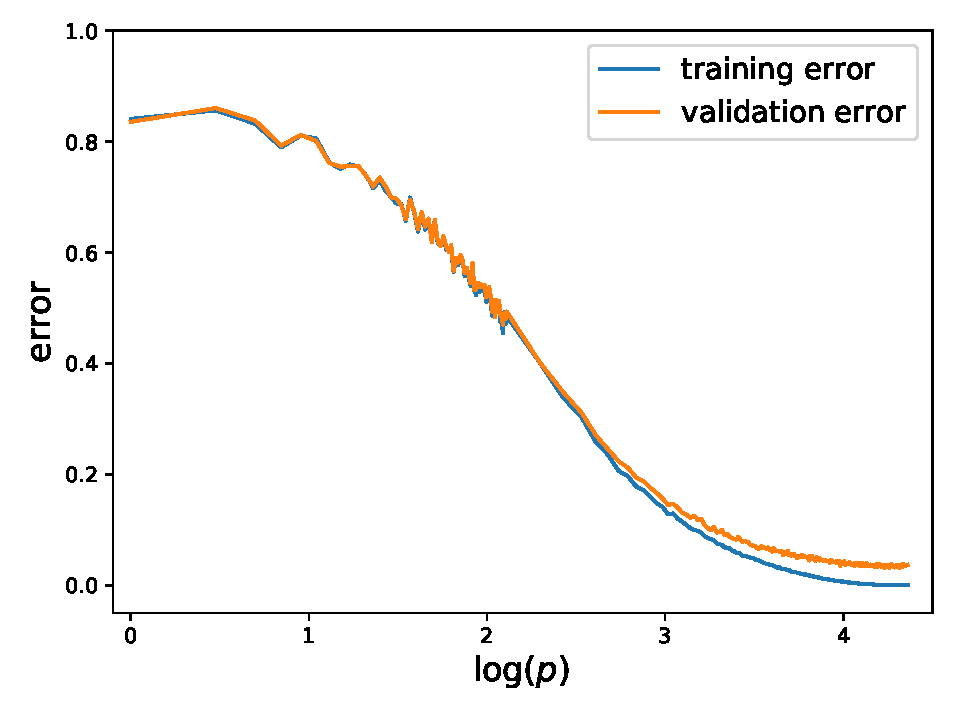
\includegraphics[width=.7\textwidth]{figures/val_plot.pdf}
		\caption{Training and validation errors for various values of $p$. (Apparent variation in noise scale is due partly to log scale and different sampling densities in different regions.)}
		\label{fig:val}
	\end{figure}

	There was no noticeable absolute minimum of validation error, and time limitations precluded exploring higher $p$ with useful resolution. (Even on Hyak, any $p > 20000$ can take $\sim$20--30 minutes to train.) Accordingly we took $p=10000$, where the validation error seems to begin leveling off, as our final value, since higher $p$ increased computation costs with little appreciable improvement in validation accuracy.



	\item We can use Hoeffding's inequality to establish a 95\% confidence interval for the test error. For a family of $m$ bounded random variables $X_i$ with expected mean $\mu$ --- in this case, the 0/1 loss for each test data point, whose expected mean is the true classification error --- it gives that for $\delta \in (0,1)$,
	%
	\begin{align}
		\mathbb{P}\left(\left|\left(\frac{1}{m}\sum_{i=1}^m X_i\right) - \mu\right| \geq \sqrt{\frac{\log(2/\delta)}{2m}}\right) &\leq \delta.
	\end{align}
	%
	In our case we take $\delta = 0.05$ and $m= 10000$ (the size of the test set) and find that with at least 95\% probability, the true error lies within 0.0136 of our measured error. Using $p=10000$ as determined above, we measure a test error of 3.99\%, so our 95\% confidence interval is $[2.63,5.35]$.
	\end{enumerate}
\end{enumerate}

\clearpage

\lstinputlisting[language=Python]{code/mnist_ridge_validate.py}

\clearpage

\lstinputlisting[language=Python]{code/mnist_ridge_test.py}

\end{document}